
\documentclass{beamer}
\usepackage{graphicx}
\usepackage{amsmath,amssymb,amstext,amsthm,xargs}
\usepackage{amsfonts}
\usepackage{bbm}
\usepackage{beamerthemesplit}

\usepackage[utf8]{inputenc}
\usepackage[french]{babel}
\usepackage{bbm}

\usetheme{Antibes}
\mode<presentation>
\useoutertheme{tree}
\usecolortheme{beaver}
\useinnertheme{rectangles}

\setbeamerfont{block title}{size={}}
%\usecolortheme[rgb={0.55,0.1,0.05}]{structure}
%\usecolortheme[rgb={0.75,0.1,0.05}]{structure}
\usepackage{color}

\newenvironment{disarray}{\everymath{\displaystyle\everymath{}}\array} {\endarray}
\newtheorem{theo}{Théorème}
\newtheorem{prop}[theo]{Proposition}
\newtheorem{conj}[theo]{Conjecture}
\newtheorem{cor}{Corollary}[theo]

\newtheorem{lem}{Lemme}
\newtheorem{nota}{Notation}
\newtheorem{rk}{Remark}
\newtheorem{exa}{Example}
\newtheorem{df}{Definition}
\newtheorem{terminologie}{Terminologie}
\def\rme{\mathrm{e}}
\def\rmi{\mathrm{i}}
\def\rset{\mathbb{R}}
\def\nset{\mathbb{N}}
\def\dlim{\stackrel{d}{\rightarrow}}
\newcommandx{\plim}[1][1=]{\stackrel{\PP_{#1}}{\longrightarrow}}
\def\iid{i.i.d.}
\def\1{\mathbbm{1}}
\newenvironment{dem}{\textbf{Proof}}{\flushright$\blacksquare$\\}
%\def\blankframe{
%\mode<presentation>{
%  { \setbeamertemplate{background canvas}[default]
%    \setbeamercolor{background canvas}{bg=black}
%    \begin{frame}[plain]{}
%    \end{frame}
%  }
%}
%\mode<presentation>{
%\setbeamertemplate{background canvas}[default]
%\setbeamercolor{background canvas}{bg=white}}
%\mode*
%}
\def\eqsp{\,}
\DeclareMathOperator{\E}{{\mathbb E}}
\def\PE{\E}
\def\PCov{\mathrm{Cov}}
\DeclareMathOperator{\F}{{\mathbb F}}
\DeclareMathOperator{\G}{{\mathbb G}}
\DeclareMathOperator{\D}{{\mathbb D}}
\DeclareMathOperator{\R}{{\mathbb R}}
\DeclareMathOperator{\C}{{\mathbb C}}
\DeclareMathOperator{\Z}{{\mathbb Z}}
\DeclareMathOperator{\N}{{\mathbb N}}
\DeclareMathOperator{\K}{{\mathbb K}}
\DeclareMathOperator{\T}{{\mathbb T}}
\DeclareMathOperator{\PP}{{\mathbb P}}
\DeclareMathOperator{\QQ}{{\mathbb Q}}
\DeclareMathOperator{\Q}{{\mathbb Q}}
\DeclareMathOperator{\IF}{{\mathbb I}}


%%%%%%%%%%%%%%%%%%%%%%%%%%%%%%% Pour le modèle lin\'eaire

\DeclareMathOperator{\bX}{\boldsymbol{X}}
\DeclareMathOperator{\bY}{\boldsymbol{Y}}
\DeclareMathOperator{\bx}{\boldsymbol{x}}
\DeclareMathOperator{\vp}{\boldsymbol{p}}
\DeclareMathOperator{\vq}{\boldsymbol{q}}
\DeclareMathOperator{\estMCNL}{\widehat \theta_n^{\,\,{\tt mcnl}}}
\DeclareMathOperator{\estMV}{\widehat \theta_n^{\,\,{\tt mv}}}
\DeclareMathOperator{\est}{\widehat \theta_{\mathnormal{n}}}
\DeclareMathOperator{\var}{\mathrm{Var}}
\def\Var{\var}
\DeclareMathOperator{\estMVc}{\widehat \theta_{n,0}^{\,{\tt mv}}}
\DeclareMathOperator{\Xbar}{\overline{\mathnormal{X}}_\mathnormal{n}}

\newcommand{\indi}[1]{\mathbbm{1}_{\{#1\}}}
\newcommand{\coint}[1]{\left[#1\right)}
\newcommand{\ocint}[1]{\left(#1\right]}
\newcommand{\ooint}[1]{\left(#1\right)}
\newcommand{\ccint}[1]{\left[#1\right]}

\definecolor{LightYell}{rgb}{0.95,0.83,0.70}
\definecolor{orange}{rgb}{1.0,0.50,0.01}
\definecolor{StroYell}{rgb}{0.95,0.88,0.72}
\definecolor{lightred}{rgb}{0.75,0.033,0}
\definecolor{shadecolor1}{rgb}{0.90,0.83,0.70}
\definecolor{myem}{rgb}{0.797,0.598,0.598}
\definecolor{BrickRed}{cmyk}{0,0.89,0.94,0.28}
\definecolor{RoyalPurple}{cmyk}{0.75,0.9,0,0}

\newcommand{\tco}[1]{\textcolor{orange}{#1}}
\newcommand{\tcr}[1]{\textcolor{lightred}{#1}}

\def\gauss{\mathcal{N}}
\def\truetheta{\theta}
\def\truebeta{\boldsymbol{\beta}}
\def\projX{A}
\def\curtheta{\alpha}
\def\argmin{\mathrm{argmin}}
\def\ie{\emph{i.e.}}
\def\regressmat{\mathbb{X}}
\def\errpred{\boldsymbol{\hat{\xi}}}
\def\bnoise{\boldsymbol{\xi}}
\def\predY{\hat{\mathbf{Y}}}
\DeclareMathOperator{\estregress}{\widehat{\truebeta}_n}
\DeclareMathOperator{\estMC}{\widehat \theta_n^{\,\,{\tt mc}}}
\def\curbeta{b}
\def\bcurbeta{\mathbf{b}}
\newcommand{\indep}{\rotatebox[origin=c]{90}{$\models$}} 
\newcommand{\Id}[1]{\mathrm{Id}_{#1}}

\title{MAP 433 : Introduction aux méthodes statistiques. Cours 8}
%\author{M. Hoffmann}
%\institute{Université Paris-Est and ETG}
\begin{document}
\date{16 Octobre 2015}
\maketitle



\begin{frame}
\frametitle{Aujourd'hui}
\tableofcontents
\end{frame}

\section{Le modèle de régression}
\begin{frame}
\frametitle{Modèle de régression}
\begin{df}
Données: $(\bx_1,Y_1),\ldots, (\bx_n,Y_n)$ avec $Y_i \in \R, \bx_i\in \R^k$, et
$$
Y_i = r(\alert{\truebeta},\bx_i)+ \sigma \xi_i,\;\;\E_{\truetheta}\big[\xi_i\big]=0,
$$
\begin{itemize}
%\item $\bx \leadsto r(\alert{\truetheta},\bx)$ fonction de \alert{ régression}, connue au paramètre
%$\truetheta$ près.
\item \alert<1>{$\bx_i$ déterministes}
\item \alert<2>{ les variables $\xi_i$ sont centrées, $\PE_{\truetheta}[\xi_i]=0$,
décorrélées, $\PE_{\truetheta}[\xi_i \xi_j]= 0$ si $i \ne j$ et de variance unité $\PE[\xi_i^2]= 1$ \alert{ (homoscédasticité)}.}
\item \alert<3>{\alert{Paramètres}: $\truetheta= (\truebeta,\sigma^2) \in  \R^d \times \R_+.$}
\end{itemize}
\end{df}


\end{frame}

\begin{frame}
\frametitle{Régression gaussienne}


\begin{itemize}
\item  \alert{Modèle de régression Gaussien}:
\tco{$$Y_i =
r({\truebeta},\bx_i)+\ \sigma \xi_i,\;\;\truetheta \in \Theta\subset  \R^d \times \rset_+.$$
}
où \tco{$\xi_i \sim \gauss(0,1)$}, i.i.d.
\item \alert{On sait expliciter la vraisemblance  de l'observation} $Z=(Y_1,\dots,Y_n)$ $\Longrightarrow$ appliquer le
principe du maximum de vraisemblance.
$$\boxed{{\mathcal L}_n(\truetheta, Y_1,\ldots, Y_n)
= \tfrac{1}{(\sqrt{2\pi \sigma^2})^{n}} \exp\Big(-\frac{1}{2\sigma^2}\sum_{i = 1}^n\big(Y_i-
r({\truebeta},\bx_i)\big)^2\Big)}$$

%d'où
%$$\PP^{(Y_1,\ldots, Y_n)}(dy_1\ldots dy_n) = \Big(\prod_{i=1}^n \frac{1}{\sqrt{2\pi \sigma^2}}\exp\big(-\frac{1}{2\sigma^2}(y-\truetheta^T\bx_i)\big)\Big) dy_1\ldots dy_n$$
\end{itemize}
\end{frame}


\begin{frame}
\frametitle{Estimateur des moindres carrés}
Maximiser la \alert{ vraisemblance} en régression gaussienne
\begin{align*}
\estregress &\in \argmin_{\bcurbeta \in \rset^k} \sum_{i = 1}^n \big(Y_i-r(\bcurbeta,\bx_i)\big)^2 \\
\hat{\sigma}_n^2 &= n^{-1} \sum_{i=1}^n (Y_i - r(\estregress,\bx_i))^2
\end{align*}
%\begin{df}
%Estimateur des \alert{moindres carrés} : tout estimateur
%$\estregress$ t.q. \centerline{$\estregress \in \arg \min_{\truebeta \in
%\Theta}\sum_{i = 1}^n \big(Y_i-r({\truebeta},\bx_i)\big)^2.$}
%\end{df}
\begin{itemize}
\item  L'estimateur $\estregress$ est appelé l'\alert{estimateur des moindres carrés}. Il peut être appliqué même dans un cas non gaussien.
\item \alert{ Existence, unicité.}
\end{itemize}
\end{frame}


\section{Régression linéaire multiple}

\begin{frame}
\frametitle{Régression linéaire multiple (=Modèle linéaire)}
\begin{itemize}
\item La fonction de régression est $r(\truebeta,\bx_i) = \bx_i^T \truebeta$.
On observe
$$(\bx_1,Y_1),\ldots, (\bx_n,Y_n)$$
avec
$$\boxed{Y_i = \bx_i^T \truebeta+ \sigma \xi_i,\;\;i=1,\ldots, n}$$
où $\truetheta \in \Theta = \R^k,\;\;\bx_i \in \R^k$.
\item \alert{Matriciellement}
$$\boxed{\bY = 
\left[
\begin{matrix}
  Y_1 \\
  Y_2 \\
  \vdots \\
  Y_n
\end{matrix}
\right]
= 
\left[
\begin{matrix}
 \bx_1^T \\
 \bx_2^T \\
 \vdots  \\
 \bx_n^T
\end{matrix}
\right]
\truebeta +
\sigma 
\left[
\begin{matrix}
 \xi_1 \\
 \xi_2 \\
 \vdots  \\
 \xi_n
\end{matrix}
\right]
=\regressmat \truebeta + \sigma \bnoise.}
$$
\end{itemize}
\end{frame}

\begin{frame}
\frametitle{EMC en régression linéaire multiple}
\begin{itemize}
\item Estimateur des \alert{moindres carrés} en régression
linéaire multiple : tout estimateur $\estregress$ satisfaisant
$$\sum_{i = 1}^n
\big(Y_i- \bx_i^T \estregress \big)^2 = \min_{\bcurbeta \in \R^k}\sum_{i =
1}^n \big(Y_i- \bx_i^T \bcurbeta\big)^2.$$
\item En notation matricielle :
\[
\|\boldsymbol{Y}-\regressmat\estregress\|^2 =   \min_{\bcurbeta \in \R^k}\|\bY -\regressmat\bcurbeta\|^2
\]
\alert{Projection orthogonale} sur
$$
\vect(\regressmat) = \{v\in \R^n: v=\regressmat \bcurbeta, \bcurbeta \in \R^k\} \eqsp.
$$
\end{itemize}
\end{frame}

% \subsection{Géometrie de l'EMC}

 \begin{frame}
\frametitle{Géométrie de l'EMC}
 \begin{itemize}
 \item L'EMC vérifie
$$\boxed{\regressmat \estregress = \projX \boldsymbol{Y}}$$
o\`u $\projX$ est le projecteur orthogonal sur $\vect(\regressmat)$.
\item Comme $ \bY - \projX \bY \perp \vect(\regressmat)$, on en déduit \alert{les équations normales} de l'EMC:
$$\boxed{\regressmat^T\regressmat {\estregress} =
\regressmat^T\boldsymbol{Y}.}$$
\item \underline{Remarques.}
  \begin{itemize}
  \item L'EMC est un $Z$-estimateur.
  \item \alert{unicité} de $\estregress$ si la matrice de Gram
  $\regressmat^T\regressmat$ est inversible (la matrice $\regressmat$ est de rang complet).
  \end{itemize}
\end{itemize}
\end{frame}

\begin{frame} \frametitle{Estimateur des moindres carrés}
\begin{prop}
Si $\regressmat^T\regressmat$ (matrice $k \times k$) inversible, alors l'EMC
$\estregress$ est \alert{unique} et
$$\boxed{\estregress = \big(\regressmat^T\regressmat\big)^{-1}\regressmat^T \boldsymbol{Y}}= \regressmat^{\#} \bY$$
\end{prop}
\begin{enumerate}
\item $\regressmat^{\#}$ \alert{pseudo-inverse} de $\regressmat$.
\item $\projX = \regressmat\big(\regressmat^T\regressmat\big)^{-1}\regressmat^T = \regressmat \regressmat^{\#}$
projecteur orthogonal sur $\vect(\regressmat)$.
\end{enumerate}
\end{frame}


\begin{frame}
\frametitle{Propriétés de l'estimateur}
\begin{theo}[Régression Gaussienne]
Supposons que   $\bY= \regressmat \truebeta + \sigma \bnoise$ avec $\bnoise \sim \gauss(0, \Id{n})$.
Alors, $\estregress \sim \gauss\left(\truebeta,\sigma^2(\regressmat^T \regressmat)^{-1}\right)$
\end{theo}
\begin{proof}
Comme $\regressmat^{\#}= (\regressmat^T \regressmat)^{-1} \regressmat^T$, $\regressmat^{\#} \regressmat = \Id{k}$. Par conséquent:
\begin{align*}
\estregress
&= \regressmat^{\#} \bY = \regressmat^{\#} (\regressmat \truebeta + \sigma \bnoise) \\
&= \truebeta + \sigma \regressmat^{\#} \bnoise
\end{align*}
Le vecteur $\regressmat^{\#} \bnoise$ est Gaussien centré de matrice de covariance
\[
\PE\left[ \regressmat^{\#} \bnoise \bnoise^T \left( \regressmat^{\#} \right)^T \right] =
\regressmat^{\#} \PE\left[ \bnoise \bnoise^T \right] \left( \regressmat^{\#} \right)^T  = \regressmat^{\#} \left( \regressmat^{\#} \right)^T = (\regressmat^T \regressmat)^{-1} \eqsp.
\]
\end{proof}
\end{frame}


\begin{frame}
\frametitle{Prédiction et Erreur de prédiction}
\begin{itemize}
\item \alert{Prédiction}
\[
\predY= \regressmat \estregress = \projX \bY
\]
projection des observations sur l'espace de régression.
\item \alert{Erreur (résidu) de prédiction}:
\[
\bY - \predY = (\Id{n} - \projX) \bY \eqsp.
\]
\item Si  $\bY= \regressmat \truebeta +  \sigma \bnoise$, alors
\tco{
\begin{align*}
\predY    &= \regressmat \truebeta + \sigma \projX \bnoise \\
\bY - \predY  &= \sigma (\Id{n}-\projX) \bnoise
\end{align*}
}
car $\projX \regressmat= \regressmat$ ($\projX$ est le projecteur orthogonal sur l'image de $\regressmat$).
\end{itemize}
\end{frame}


\begin{frame}
\frametitle{Théorème de Cochran}
\begin{theo}
\alert{Hypothèses}
\begin{itemize}
\item $\bY \sim \gauss(\mu,\sigma^2 \Id{n})$,
\item $\mathcal{M}$ un sous espace de $\R^n$ de dimension $k$,
\item $\Pi$ la matrice de projection orthogonale
sur $\mathcal{M}$ et $\Pi_{\perp}= \Id{n} - \Pi$ la matrice de projection orthogonale sur $\mathcal{M}^\perp$.
\end{itemize}
Alors
\begin{enumerate}
\item \alert<1>{$\Pi \bY \sim \gauss(\Pi \mu, \sigma^2 \Pi)$, $\Pi_\perp \bY \sim \gauss(\Pi_{\perp} \mu, \sigma^2 \Pi_{\perp})$}
\item \alert<2>{les vecteurs $\Pi \bY$ et $\Pi_\perp \bY$ sont indépendants}
\item \alert<3>{$\| \Pi(\bY - \mu) \|^2 / \sigma^2 \sim \chi^2_k$ et $\Pi_\perp(\bY-\mu) \|^2/\sigma^2 \sim \chi^2_{n-k}$}.
\end{enumerate}
\end{theo}
\end{frame}

\begin{frame}
\frametitle{Résidus et variance résiduelle}
\alert{Hypothèse:} $\bY= \regressmat \truebeta +  \sigma \bnoise$, $\bnoise \sim \gauss(0,\Id{n})$.
\begin{align*}
\estregress    &=  \truebeta + \sigma \regressmat^{\#} \bnoise \\
\bY - \predY   &=  (\Id{n}-\projX) \bY = \sigma (\Id{n} - \projX) \bnoise \quad \text{car $(\Id{n} - \projX) \projX= 0$} \\
\hat{\sigma}_n^2 &= (n-k)^{-1} \| \bY - \predY \|^2
\end{align*}
\begin{theorem}
\begin{enumerate}
\item $(n-k) \hat{\sigma}_n^2/\sigma^2$ suit une loi du $\chi^2$ à $(n-k)$ degrés de liberté.
\item $\estregress$ et $\hat{\sigma}_n^2$ sont indépendants.
\end{enumerate}
\end{theorem}
\begin{proof}
\only<1>{
$(\Id{n}- \projX) \bnoise \sim \gauss(0,(\Id{n}-\projX))$ et donc $\|(\Id{n}- \projX) \bnoise\|^2$ suit une loi du $\chi^2$ à
$(n-k)= \mathrm{Tr}(\Id{n} - \projX)$ d.l.
}
\only<2>{
$$
\estregress= \truebeta +  \sigma \regressmat^{\#} \bnoise = \truebeta + \sigma \regressmat^{\#} \projX \bnoise \quad \bY - \predY= \sigma (\Id{n} - \projX) \bnoise
$$
Par le théorème de Cochran, $ \projX \bnoise$ et $(\Id{n}- \projX) \bnoise$ sont indépendants.
}
\end{proof}
\end{frame}

\begin{frame}
\frametitle{Loi de Student}
\begin{definition}
Soit $Z$ une variable aléatoire de loi normale centrée et réduite et soit $U$ une variable indépendante de $Z$ et distribuée suivant la loi du
$\chi^2$ à $p$ degrés de liberté. La variable
\[
T = \frac{Z}{\sqrt{U/p}}
\]
suit une loi de Student à $p$ degrés de liberté.
\end{definition}
\end{frame}

\begin{frame}
\frametitle{Loi de Fisher}
\begin{definition}
 Soient $U_1$ et  $U_2$ deux variables aléatoires indépendantes distribuées  selon des lois du $\chi^2$ à $d_1$ et $d_2$ degrés de liberté. La variable
\[
 \frac{U_1/d_1}{U_2/d_2}
\]
est distribuée suivant une loi de Fisher à $(d_1,d_2)$ d.l.
\end{definition}
\end{frame}

\begin{frame}
\frametitle{Intervalle de confiance}
\begin{theo}
\alert{Hypothèse:} $\bY= \regressmat \truebeta + \sigma \bnoise$, $\bnoise \sim \gauss(0,\Id{n})$.

Pour $j=1,\dots,k$,
\[
T_j= \frac{\hat{\beta}_j- \beta_j}{\hat{\sigma}_n\sqrt{[(\regressmat^T \regressmat)^{-1}]_{j,j}}} \sim  \mathcal{T}_{n-k}
\]
$\mathcal{T}_{n-k}$: Loi de \alert{Student} à $n-k$ d.d.l.
\end{theo}
\begin{proof}
\begin{itemize}
\item $\hat{\beta}_j- \beta_j \sim \gauss(0, \sigma^2[(\regressmat^T \regressmat)^{-1}]_{j,j})$
\item $(n-k) \hat{\sigma}_n^2/\sigma^2$ $\chi^2(n-k)$ d.l.
\item $\hat{\beta}_j- \beta_j$ et $(n-k) \hat{\sigma}_n^2$ sont indépendants.
\end{itemize}
\end{proof}
\end{frame}

\begin{frame}
\frametitle{Régions de confiance}
\begin{theo}
\alert{Hypothèse:} $\bY= \regressmat \truebeta + \sigma \bnoise$, $\bnoise \sim \gauss(0,\Id{n})$.


Soit $R$ une matrice ($q \times k$) de rang $q$ ($q \leq k$) alors
\[
\frac{1}{q \hat{\sigma}_n^2} (R\{\estregress-\truebeta\})^T \left[ R (\regressmat^T \regressmat)^{-1} R^T \right]^{-1} R\{\estregress-\truebeta\}
\sim \mathcal{F}_{q,n-k}
\]
$\mathcal{F}_{q,n-k}$: Loi de Fisher à $(q,n-k)$-d.d.l.
\end{theo}

\begin{proof}
\begin{itemize}
\item $R\{\estregress-\truebeta\} \sim \gauss( 0, \sigma^2  R (\regressmat^T \regressmat)^{-1} R^T)$ car $\estregress \sim \gauss(\truebeta,\sigma^2 (\regressmat^T \regressmat)^{-1})$
\item $(n-k) \hat{\sigma}_n^2/\sigma^2$ suit une loi du $\chi^2$ à $(n-k)$-d.l.
\item $\estregress-\truebeta$ et $\hat{\sigma}_n^2$ sont indépendants.
\end{itemize}
\end{proof}
\end{frame}

\begin{frame}
\frametitle{Intervalles de confiance}
\begin{theo}
\begin{enumerate}
\item Un intervalle de confiance bilatéral de niveau $1-\alpha$,  pour un $\beta_{j}$, $j=1,\dots, p$, est donné  par
    $$
    [\hat{\beta}_{j}-t_{n-p}(1-\alpha/2)\hat{\sigma}_n\sqrt{[(X^T X)^{-1}]_{jj}},\ \hat{\beta}_{j}+t_{n-p}(1-\alpha/2)\hat{\sigma}_n\sqrt{[(X^T X)^{-1}]_{jj}}]
    $$
\item Un intervalle de confiance bilatéral de niveau $ 1-\alpha$, pour $\sigma^{2}$  est donné par
$$
\ccint{\frac{(n-p)\hat{\sigma}_n^{2}}{c_{2}},\ \frac{(n-p)\hat{\sigma}_n^{2}}{c_{1}}}\ \quad \text{où} \quad  \PP(c_{1}\leq\chi_{n-p}^{2}\leq c_{2})=1-\alpha.
$$
\end{enumerate}
\end{theo}
\end{frame}


\begin{frame}
\frametitle{Régions de confiance}
\begin{theo}
 Une région de confiance  pour $q$ ($q\leq k$)  param\`{e}tres $\beta_{j}$ notés $(\beta_{j_{1}},\ \cdots,\ \beta_{j_{q}})$ de niveau
 $ 1-\alpha$ est donn\'{e}e  par
\begin{multline*}
\Big\{(\beta_{j_1},\dots,\beta_{j_q}) \rset^q, \\ \frac{1}{q\hat{\sigma}_n^{2}}[E(\estregress-\truebeta)]^T[E(X^TX)^{-1}E^T]^{-1}[E(\estregress-\truebeta)]\leq f_{q,n-p}(1-\alpha)\Big\},
\end{multline*}
o\`{u}
\begin{itemize}
\item $E$ est la matrice de taille $q\times k$ telle que
$$
\left[
\begin{matrix}
  \beta_{j_1} \\
  \vdots \\
  \beta_{j_q}
\end{matrix}
\right]
= E \truebeta
$$
(tous les éléments sont nuls sauf les $[E]_{ij_{i}}$, $i=1,\dots,q$ qui valent 1)
\item $f_{q,n-k}(1-\alpha)$ est le quantile de niveau $(1-\alpha)$ d'une loi de Fisher admettant $(q,\ n-k)$ d.d.l.
\end{itemize}
\end{theo}
\end{frame}

\begin{frame}
\frametitle{Un exemple}
\begin{figure}
  \centering
  % Requires \usepackage{graphicx}
  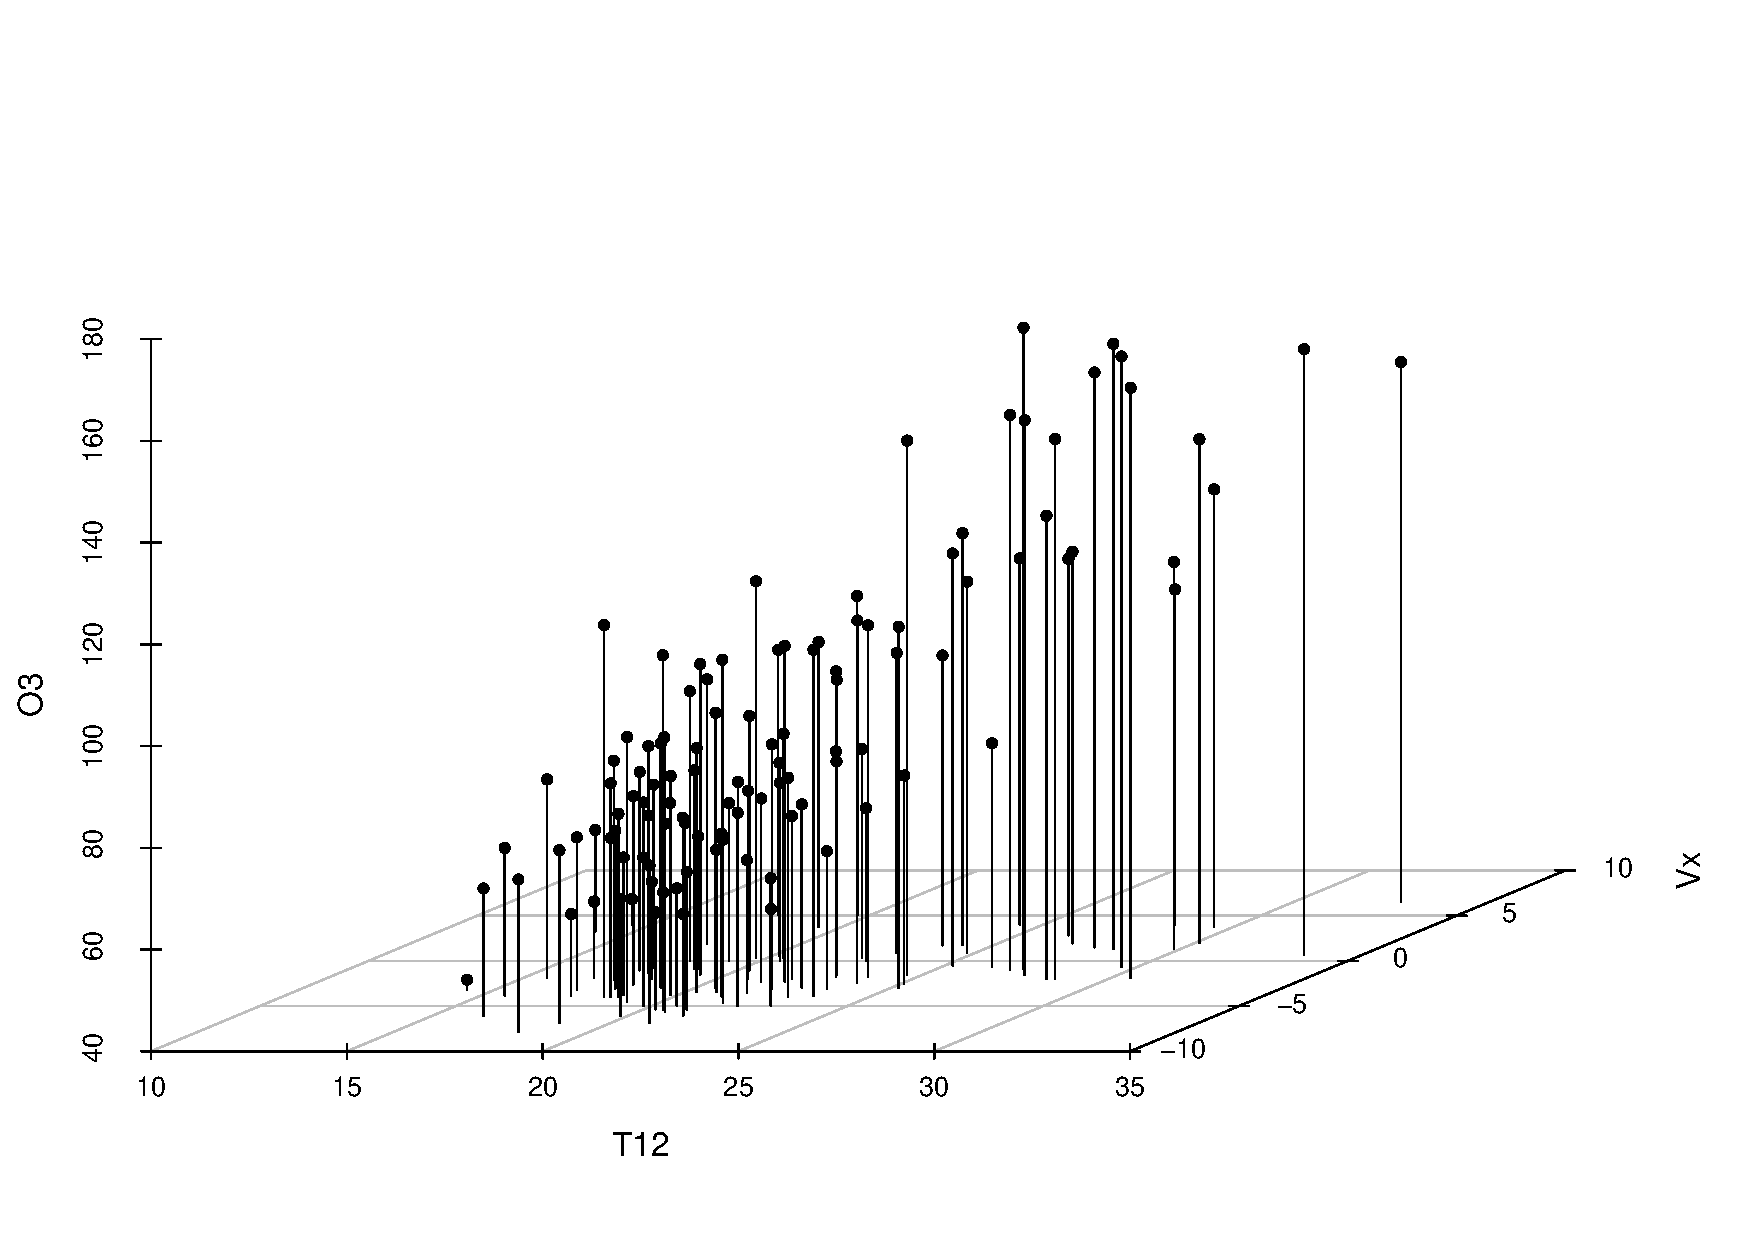
\includegraphics[width=0.8\textwidth]{ScatterPlot}\\
  \caption{Représentation brute des données: modèle d'explication de l'ozone (O3) par la température à 12h (T12) et le Vent à 12h (Vx12)}
\end{figure}
\end{frame}

\begin{frame}
\frametitle{Régression multiple}
\alert{Modèle de régression}
\[
\mathrm{maxO3}= \beta_1 + \beta_2 \mathrm{T12} + \beta_3 \mathrm{Vx12} + \beta_4 \mathrm{Ne12} + \sigma \bnoise
\]
\alert{Intervalles de confiance}
\begin{table}
\begin{tabular}{ccc}
            &      2.5 \% &   97.5 \% \\
(Intercept) &-25.4886483  & 33.280203 \\
T12         &  3.4819098  & 5.544563  \\
Vx12        &  0.3264694  & 2.931560  \\
Ne12        & -3.6368523  & 0.399082
\end{tabular}
\end{table}
\end{frame}

\begin{frame}
\frametitle{Régions de confiance}
\begin{figure}
  \centering
  % Requires \usepackage{graphicx}
  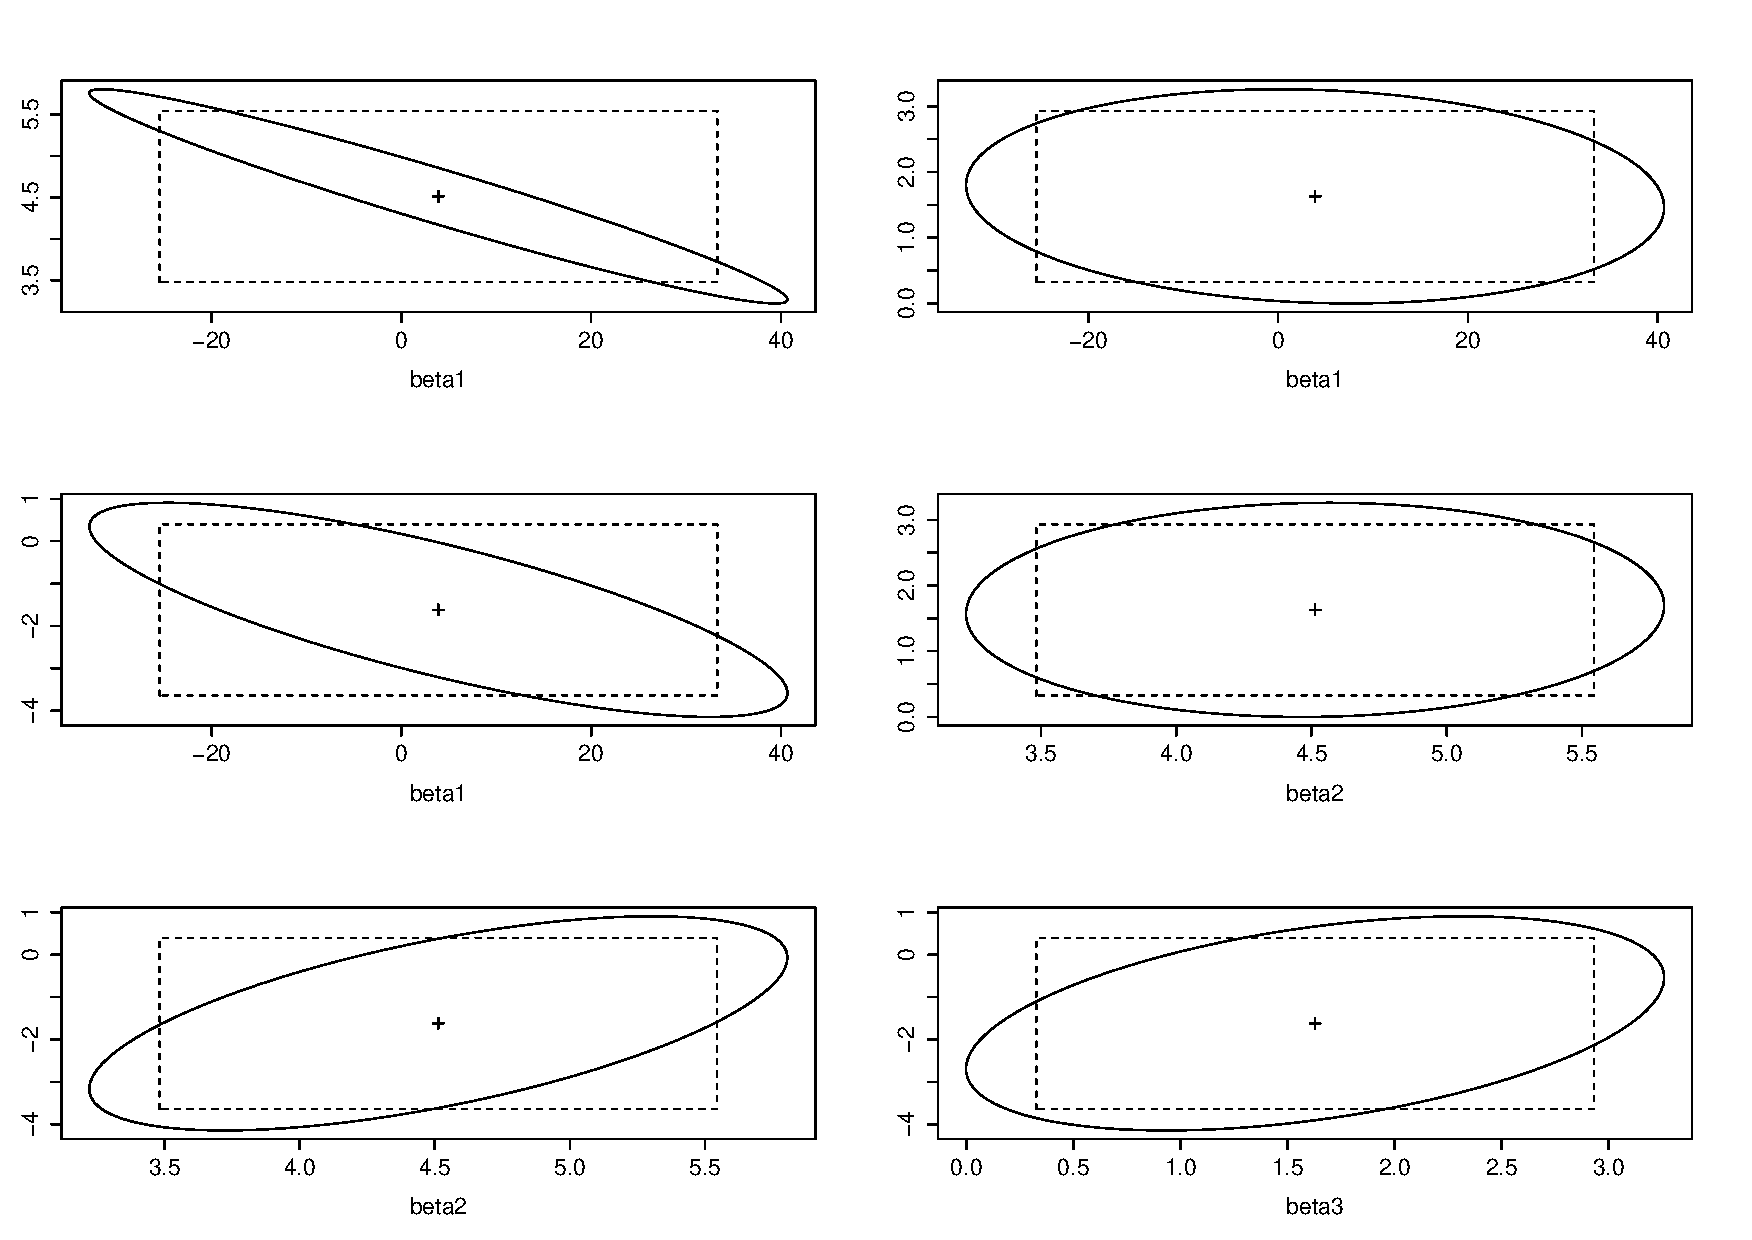
\includegraphics[width=0.8\textwidth]{Rconfiance}\\
  \caption{Régions de confiance et rectangle des couples de paramètres}
\end{figure}
\end{frame}

\section{Choix de modèles}

\begin{frame}
\frametitle{Problème}
Nous avons modélisé les pics d'ozone par $\mathrm{T12}$, $\mathrm{Vx12}$ et $\mathrm{Ne12}$.
Il para\^{i}t raisonnable de se poser les questions suivantes :
\begin{enumerate}
\item Est-ce que la valeur de $\mathrm{O3}$ est influenc\'{e}e par $\mathrm{Vx}$?
\item Y a-t-il un effet n\'{e}bulosit\'{e}?
\item Est-ce que la valeur de $\mathrm{O3}$ est influenc\'{e}e par $\mathrm{Vx}$ ou $\mathrm{T12}$ ?
\end{enumerate}
Rappelons que le mod\`{e}le utilis\'{e} est le suivant:
\[
\mathrm{O3}= \beta_1 + \beta_2 \mathrm{T12} + \beta_3 \mathrm{Vx12} + \beta_4 \mathrm{Ne12} + \sigma \bnoise
\]
Nous pouvons expliciter les trois questions pr\'{e}c\'{e}dentes en terme de test d'hypo- th\`{e}se :
\begin{enumerate}
\item correspond \`{a} $\mathrm{H}_{0}:\beta_{3}=0$, contre $\mathrm{H}_{1}$ : $\beta_{3}\neq 0$;
\item  correspond \`{a} $\mathrm{H}_{0}$ : $\beta_{4}=0$, contre $\mathrm{H}_{1}$ : $\beta_{4}\neq 0$;
\item correspond \`{a} $\mathrm{H}_{0}$ : $\beta_{2}=\beta_{3}=0$, contre $\mathrm{H}_{1}$ : $\beta_{2}\neq 0$ ou $\beta_{3}\neq 0$.
\end{enumerate}
\end{frame}

\begin{frame}
\frametitle{Test entre mod\`{e}les embo\^{i}t\'{e}s}
\begin{itemize}
\item \alert{Modèle}:
$$
\text{
$\bY=\regressmat\truebeta+ \sigma \bnoise$ o\`{u} $\bnoise \sim \gauss(0,\ \sigma^{2}\Id{n})$ \eqsp,
}
$$
ce qui implique
$$ \PE_{\truebeta,\sigma^2}[\bY]= \regressmat \truebeta \in \vect(\regressmat) \eqsp.
$$
\item On cherche à tester si
$$\PE_{\truebeta,\sigma^2}[\bY] \in \vect(\regressmat_0)
$$
où $\vect(\regressmat_0) \subset \vect(\regressmat)$ est un sous espace linéaire (strict) de $\vect(\regressmat)$
\item \alert{Exemple typique:} $\mathrm{H}_0$: $\beta_{j_1} = \dots = \beta_{j_q}= 0$. Dans ce cas, $\regressmat_0$ sont les colonnes
de la matrice $\regressmat$ qui correspondent aux indices $\{1,\dots,k\} \setminus \{j_1,\dots,j_q\}$
\end{itemize}
\end{frame}


\begin{frame}
\frametitle{Test du rapport de vraisemblance généralisé}
\[
\Lambda_n = \frac{\sup_{(\truebeta_0,\sigma^2)} (2 \pi \sigma^2)^{-n/2} \exp(-1/(2\sigma^2) \| \bY - \regressmat_0 \truebeta_0\|^2)}{\sup_{(\truebeta,\sigma^2)} (2 \pi \sigma^2)^{-n/2} \exp(-1/(2\sigma^2) \| \bY - \regressmat \truebeta\|^2)}
\]
\only<2>
{
\begin{itemize}
\item On calcule d'abord l'EMV sous le modèle contraint
\[
\bY = \regressmat_0 \truebeta_0 + \sigma \bnoise \eqsp.
\]
\item \alert{régresseur} $\estregress_0= \regressmat_0^{\#} \bY$, \alert{variance} $\hat{\sigma}_n^2= n^{-1} \| \bY - \regressmat_0 \estregress_0\|^2$
\item \alert{vraisemblance}
\[
\sup_{(\truebeta_0,\sigma^2)} (2 \pi \sigma^2)^{-n/2} \exp(-1/(2\sigma^2) \| \bY - \regressmat_0 \truebeta_0\|^2)
= \frac{exp(-n)}{(2 \pi n^{-1} \| \bY - \regressmat_0 \estregress_0\|^2)^{n/2}}
\]
\end{itemize}
}
\only<3>
{
\begin{itemize}
\item On calcule ensuite l'EMV sous le modèle non contraint
\pause \item \alert{régresseur} $\estregress= \regressmat^{\#} \bY$, \alert{variance} $\hat{\sigma}_n^2= n^{-1} \| \bY - \regressmat \estregress\|^2$
\pause \item \alert{vraisemblance}
\[
\sup_{(\truebeta,\sigma^2)} (2 \pi \sigma^2)^{-n/2} \exp(-1/(2\sigma^2) \| \bY - \regressmat \truebeta\|^2)
= \frac{exp(-n)}{(2 \pi n^{-1} \| \bY - \regressmat \estregress \|^2)^{n/2}}
\]
\end{itemize}
}
\only<4>
{
\begin{itemize}
\item En posant $\predY= \regressmat \estregress$ et $\predY_0= \regressmat_0 \estregress_0$, le RVG est donné par
\begin{align*}
\Lambda_n &= \frac{\| \bY - \predY \|^n}{\| \bY - \predY_0 \|^n}
\end{align*}
\pause \item $\predY - \predY_0 \in \vect(\regressmat)$ car $\predY \in \vect(\regressmat)$ et $\predY_0 \in \vect(\regressmat_0) \subset \vect(\regressmat)$
\pause \item $\bY - \predY \perp \vect(\regressmat)$ car $\predY= \projX \bY$ est la projection orthogonale de $\bY$ sur $\vect(\regressmat)$,
\pause \item \alert{Conclusion}
\[
\| \bY - \predY_0 \|^2 = \|\bY - \predY \|^2 + \| \predY - \predY_0 \|^2
\]
\end{itemize}
}
\only<5>{
\begin{itemize}
\item On considère la statistique de test
\[
F_n = \frac{\|\predY - \predY_0\|^2/q}{\| \bY - \predY\|^2/(n-k)}
\]
\item Le test du RVG s'écrit donc
\[
\Lambda_n = \left(1 + \{q/(n-k)\}F_n\right)^{-n/2}
\]
\item On rejette H0 si $\Lambda_n$ est inférieur à un seuil ce qui revient à tester que $F_n > d$.
\end{itemize}
}
\end{frame}

\begin{frame}
\frametitle{Distribution du test}
\alert{Modèle général (sans contrainte)}:
\[
\bY= \regressmat \truebeta + \sigma \bnoise
\]
\begin{itemize}
\item Comme $\predY = \projX \bY$ et $\predY_0= \projX[\regressmat_0] \bY$ et $\projX \projX[\regressmat_0]= \projX[\regressmat_0] \projX= \projX[\regressmat_0]$,
\begin{align*}
\predY - \predY_0&= \regressmat \truebeta + \sigma \projX \bnoise - \projX[\regressmat_0] \regressmat \truebeta + \sigma \projX[\regressmat_0] \bnoise \\
&= (\regressmat \truebeta - \projX[\regressmat_0] \regressmat \truebeta) + \sigma \projX (\Id{n} - \projX[\regressmat_0]) \bnoise \eqsp,
\end{align*}
\item D'autre part, comme $\bY - \predY$
\[
\bY - \predY= \sigma (\Id{n} - \projX) \bnoise \eqsp.
\]
\item Par le théorème de Cochran, $\projX(\Id{n} - \projX[\regressmat_0]) \bnoise$ et $(\Id{n} - \projX) \bnoise$ sont \alert{indépendants}
\item \alert{Conclusion:} Le numérateur et le dénominateur de la statistique de test sont \alert{indépendants}
\[
F_n = \frac{\|\predY - \predY_0\|^2/q}{\| \bY - \predY\|^2/(n-k)}
\]
\end{itemize}
\end{frame}

\begin{frame}
\frametitle{Distribution du test sous l'hypothèse nulle}
\begin{itemize}
\item \alert{Hypothèse nulle}: $\regressmat \truebeta = \projX[\regressmat_0] \regressmat \truebeta$ car $\regressmat \truebeta \in \vect(\regressmat_0)$.
\item \alert{Conséquence}: sous $\mathrm{H}_0$,
\[
\predY - \predY_0 =  \sigma \projX (\Id{n} - \projX[\regressmat_0]) \bnoise
\]
\item \alert{Conclusion}: par le Théorème de Cochran,  sous $\mathrm{H}_0$,
$$
\| \predY - \predY_0 \|^2/ \sigma^2
$$
est distribué suivant une variable de $\chi^2$  à $q$ d.d.l., qui est le nombre de coefficients nuls.
\end{itemize}
\end{frame}

\begin{frame}
\frametitle{Distribution du test sous l'hypothèse nulle}
\begin{itemize}
\item $(\bY - \predY)$ est indépendant de $\predY - \predY_0$ et $\| \bY - \predY \|^2/ \sigma^2$ est distribué suivant une loi du $\chi^2$ à $(n-k)$ d.d.l.
\item Sous l'hypothèse $\mathrm{H}_0$, $\| \predY - \predY_0 \|^2/\sigma^2$ et $\| \bY - \predY \|^2$ sont \alert{indépendants} et distribués suivant des lois du $\chi^2$ à \alert{$q$} et \alert{$n-k$} d.d.l.
\item \alert{Conclusion}  Sous l'hypothèse $\mathrm{H}_0$, la statistique de test est donc distribuée suivant \alert{un loi de Fisher} à $(q,n-k)$ d.d.l
\end{itemize}
\end{frame}

\begin{frame}
\frametitle{Synthèse Test entre mod\`{e}les emboît\'{e}s}
\begin{itemize}
\item Considérons l'hypothèse  nulle : $\mathrm{H}_0$: $\regressmat \truebeta \in \vect(\regressmat_0)$ (où $\vect(\regressmat_0)$ est un sous-espace vectoriel de $\vect(\regressmat)$).
\item \alert{Test:} On rejette $\mathrm{H}_0$ si
\alert{
\[
\frac{\|\predY - \predY_0\|^2/q}{\|\bY - \predY\|^2/(n-k)} \geq f_{1-\alpha}(q,n-k)
\]
}
où $f_{1-\alpha}(q,n-k)$ est le quantile $1-\alpha$ d'une loi de Fisher à $(q,n-k)$-d.d.l.
\end{itemize}
\end{frame}

\begin{frame}
\frametitle{Test de Student}
\begin{itemize}
  \item Dans le cas où $\mathrm{H}_0$: $\beta_j=0$, pour $j \in \{1,\dots,k\}$, le test est équivalent au test de Student
  \alert{
  \[
  T_j = \frac{\hat{\beta}_j}{\hat{\sigma}_n\sqrt{[(\regressmat^T\regressmat)^{-1}]_{i,i}}}
  \]
  }
  \item Sous $\mathrm{H}_0$, $T_j$ est distribué suivant une loi de Student à $(n-p)$-d.d.l
  \item Le test rejette $\mathrm{H}_0$ si
  \[
  |T_j| \geq t_{n-k}(1-\alpha/2)
  \]
  où $t_{n-k}(1-\alpha/2)$ est le quantile d'ordre $1-\alpha/2$ de la loi de Student à $(n-p)$-d.d.l.
\end{itemize}
\end{frame}

\section{Analyse des résidus}
\begin{frame}
\frametitle{Les différents résidus}
\begin{itemize}
\item Les résidus théoriques $\bY - \regressmat \truebeta$ sont estimés par
$$
\bY - \predY = \bY - \projX \bY = \sigma \projX \bnoise.
$$
\item \alert{Absence de bias}  $\PE_{\truebeta,\sigma^2}[\bY- \regressmat \truebeta]= 0$ et
$\PE_{\truebeta,\sigma^2}[(\bY - \predY)]=0$.
\item \alert{Covariance} $\PE_{\truebeta,\sigma^2}[(\bY- \regressmat \truebeta) (\bY -\regressmat \truebeta)^T]= \sigma^2 \Id{n}$ mais
\[
\PE_{\truebeta,\sigma^2}[ (\bY - \predY) (\bY - \predY)^T] = \sigma^2 (\Id{n} - \projX) \eqsp.
\]
\only<1>{\item \alert{Résidus standardisés:} Pour $i \in \{1,\dots, n\}$, nous avons:
\[
t_i = \frac{Y_i - \hat{Y}_i}{\hat{\sigma}_n \sqrt{1-\pi_{i,i}}} \eqsp, \quad \pi_{i,i}= \left[ \projX \right]_{i,i}
\]
La loi de ces résidus est difficile à calculer car le \alert{numérateur} et le \alert{dénominateur} sont dépendants.
}
\only<2>{
\item \alert{Résidus studentisés:}
\alert{
\[
t_{n,i}^*= \frac{Y_i - \hat{Y}_i}{\hat{\sigma}_{n,(i)} \sqrt{1-\pi_{i,i}}} \eqsp, \quad \pi_{i,i}= \left[ \projX \right]_{i,i} \eqsp.
\]
}
où \tco{$\hat{\sigma}_{n,(i)}$} est l'estimateur de la variance du modèle linéaire, \alert{privé de l'observation $i$}.
}
\end{itemize}
\end{frame}


\begin{frame}
\frametitle{Distribution des résidus studentisés}
\begin{theo}
Si la matrice $\regressmat$ est de rang $k$ et $\bnoise \sim \gauss(0,\Id{n})$ alors le résidu studentisé
\[
t_{n,i}^*= \frac{Y_i - \hat{Y}_i}{\hat{\sigma}_{n,(i)} \sqrt{1-\pi_{i,i}}} \eqsp, \quad \pi_{i,i}= \left[ \projX \right]_{i,i} \eqsp,
\]
est distribué suivant une loi de Student à $(n-k-1)$ d.d.l
\end{theo}
\end{frame}

\begin{frame}
\begin{figure}
  \centering
  \includegraphics[width=0.8\textwidth]{ice_cap}
\end{figure}
\end{frame}

\begin{frame}
\begin{figure}
  \centering
  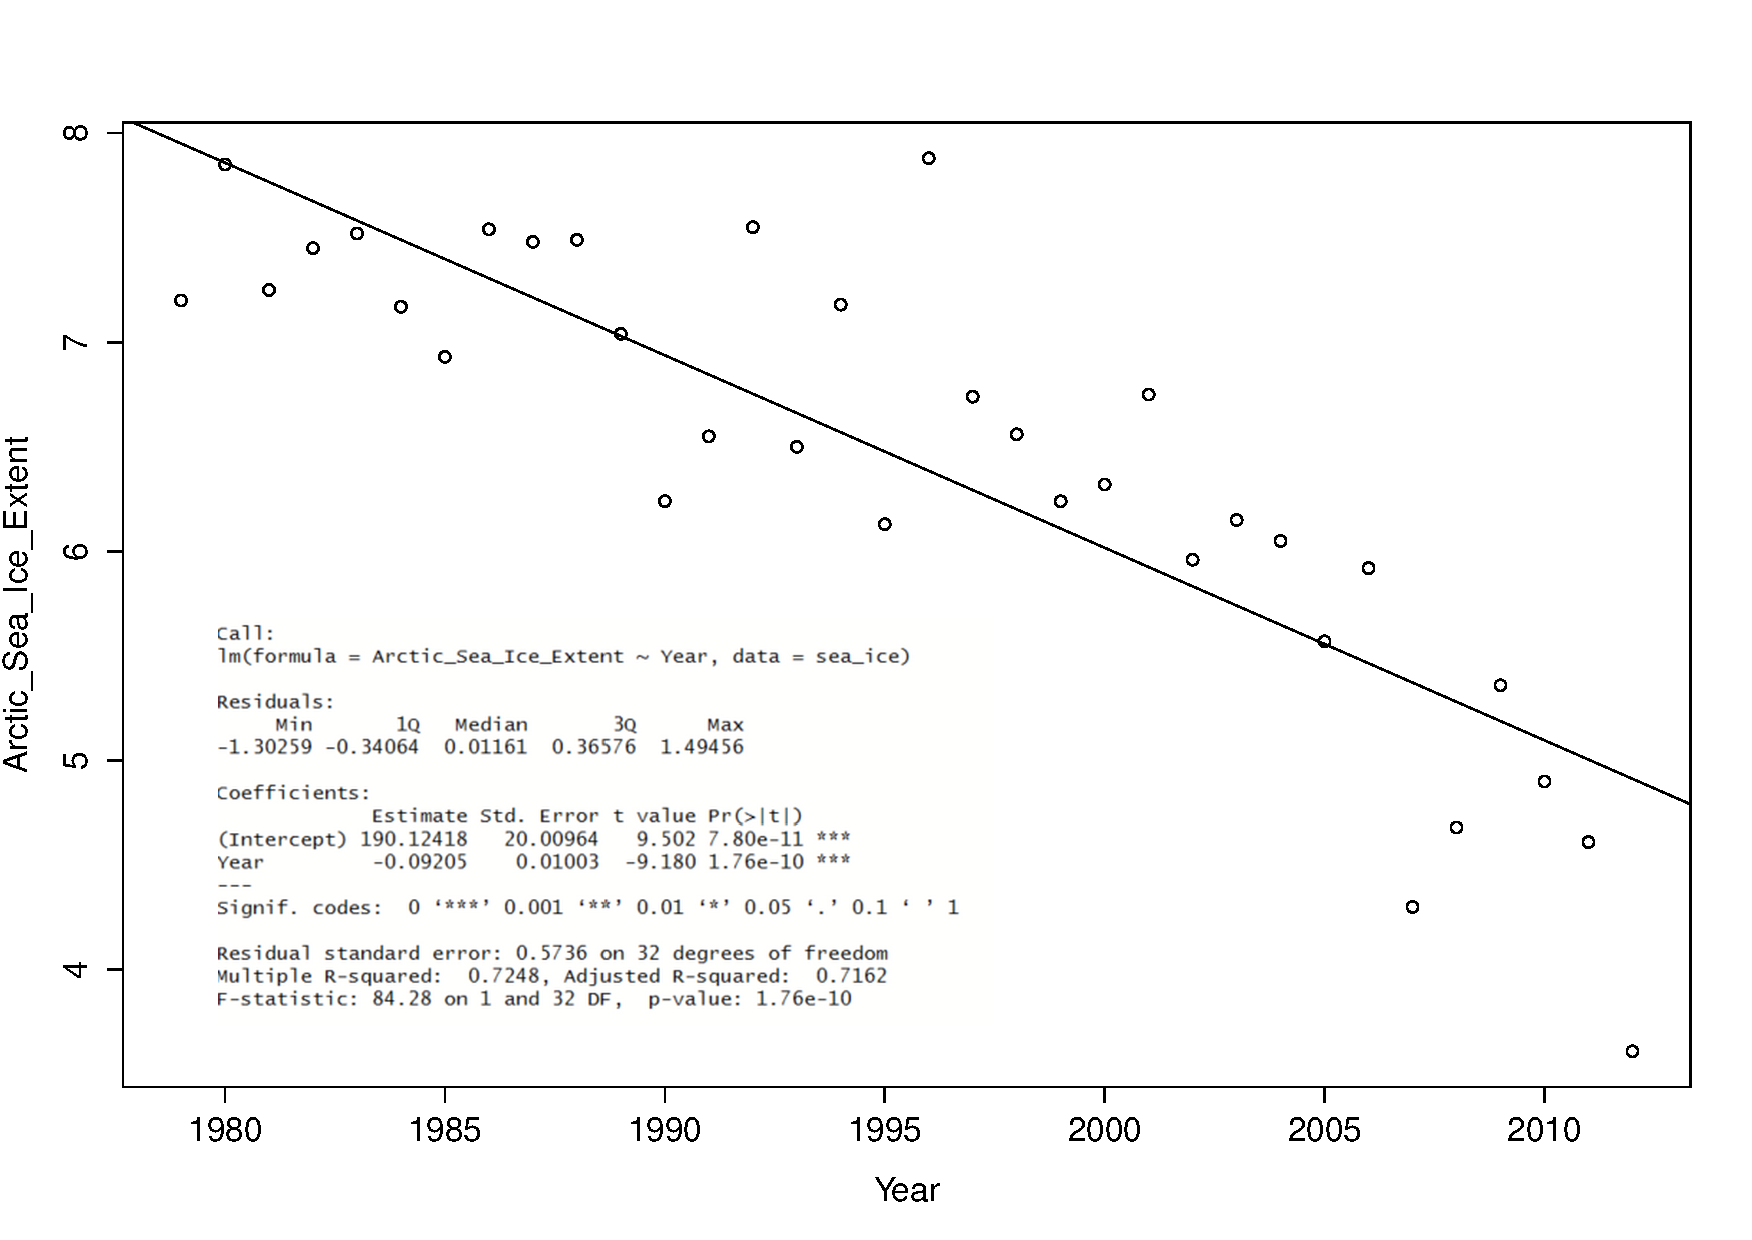
\includegraphics[width=0.8\textwidth]{sea_ice_over}
\caption{Une pente de -0.0921 montre que la surface de la banquise de 1979-2012 a perdu 92,100 $\mathrm{km}^2$. C'est à peu près 1/5 de la surface de la France qui disparaît chaque année}
\end{figure}
\end{frame}

\begin{frame}
\frametitle{la régression est elle-constante ?}
\begin{table}
\begin{tabular}{c|c|c|c}
Début & Fin & cste  & pente \\ \hline \hline\\
1979 &2001&98.3&0.0459\\
1979 &2002&108.5&0.0510\\
1979 &2003 &112.0&0.0528\\
1979 &2004 &115.6&0.0546\\
1979 &2005 &125.2&0.0594\\
1979 &2006 &126.8&0.0602 \\
1979 &2007 &149.5&0.0716 \\
1979 &2008 &162.2&0.0780 \\
1979 &2009 &163.4&0.0786 \\
1979 &2010 &168.8&0.0813 \\
1979 &2011 &175.4&0.0847 \\
1979 &2012 &190.1&0.0921 \\
\end{tabular}
\caption{La pente semble croître lorsque l'on augmente l'horizon temporel}
\end{table}
\end{frame}

\begin{frame}
\frametitle{Résidus standardisés}
\begin{figure}
  \centering
  \includegraphics[width=0.8\textwidth]{Studentized_Residuals}
  \caption{Les résidus studentisés sont négatifs en début et en fin de périodes: suspicion d'un effet non-linéaire}
\end{figure}
\end{frame}

\begin{frame}
\frametitle{Modèle quadratique}
\begin{figure}
  \centering
  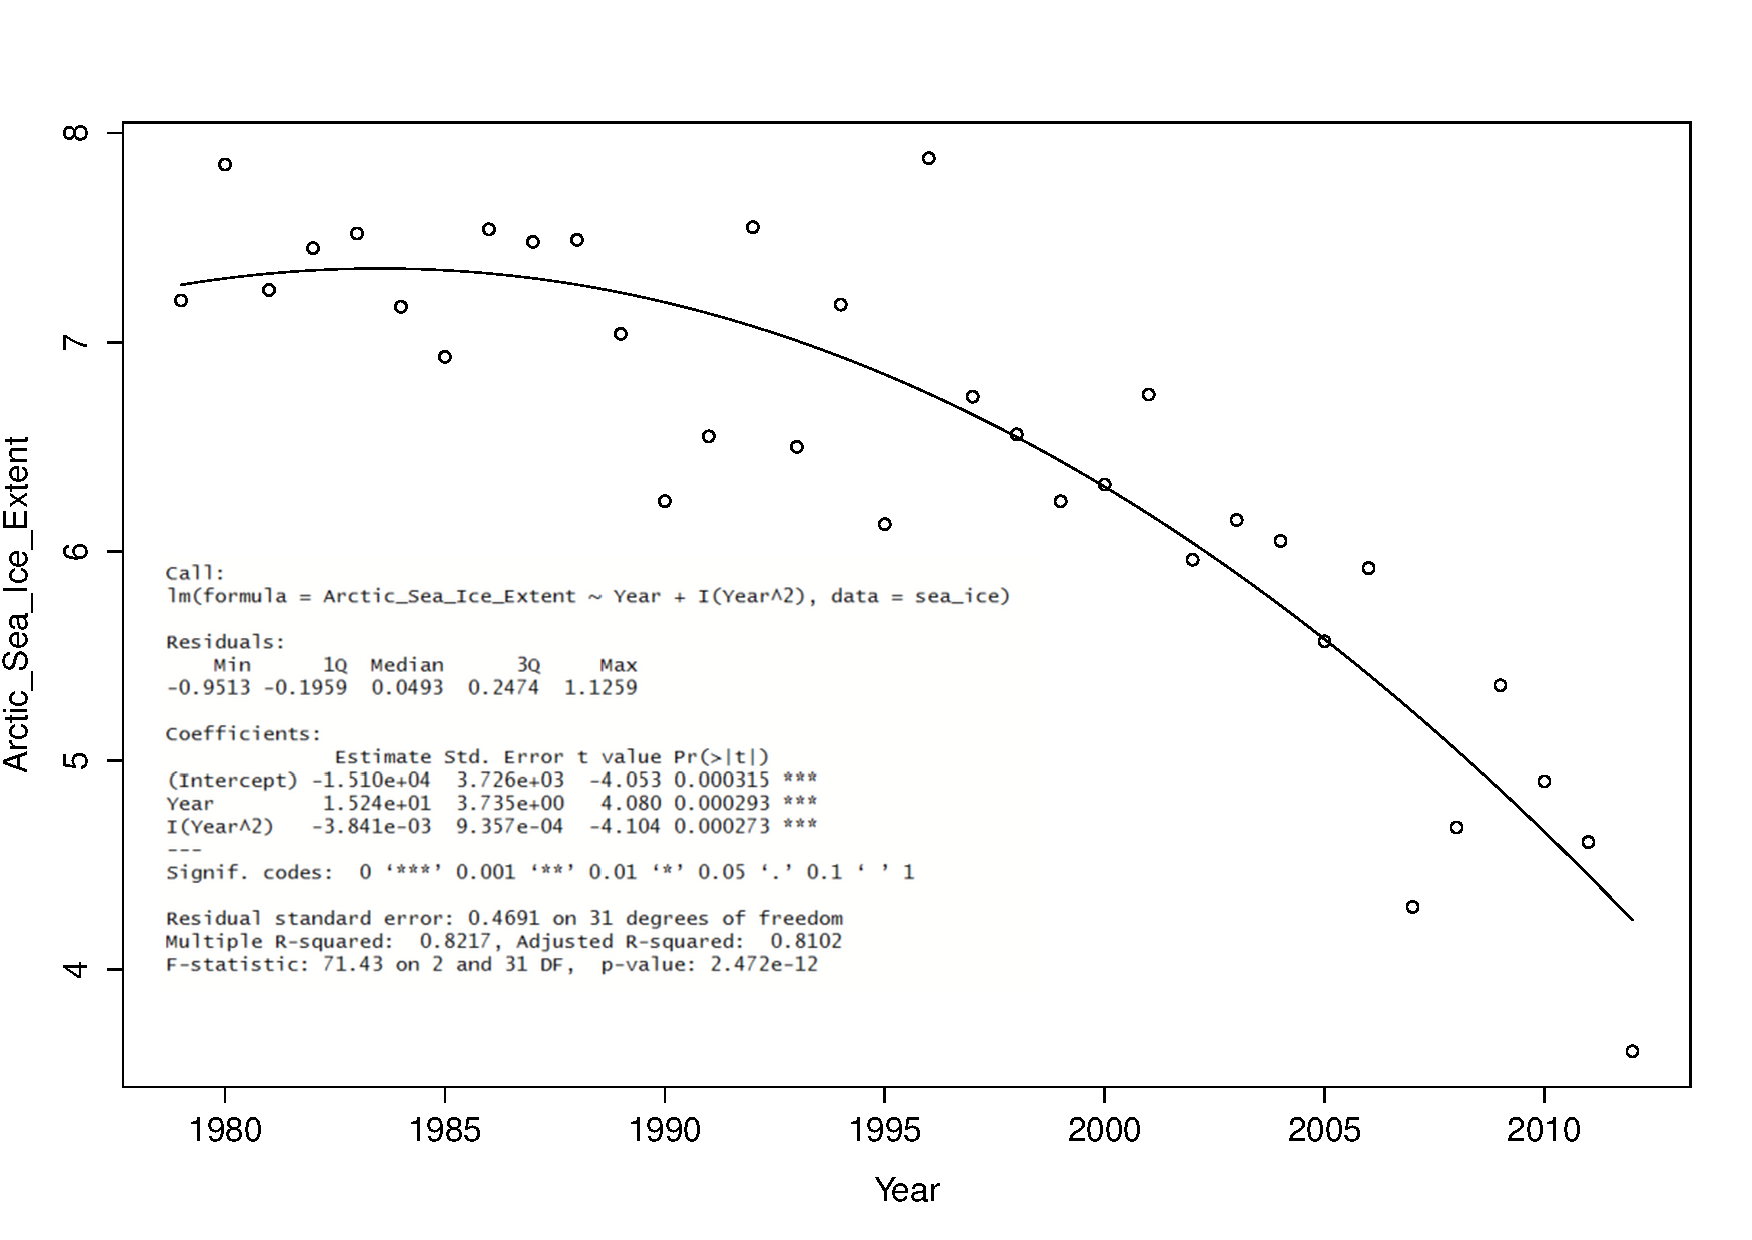
\includegraphics[width=0.8\textwidth]{sea_ice_quadratic}
  \caption{Ajustement quadratique}
\end{figure}
\end{frame}

\begin{frame}
\frametitle{Choix de modèles}
\begin{figure}
  \centering
  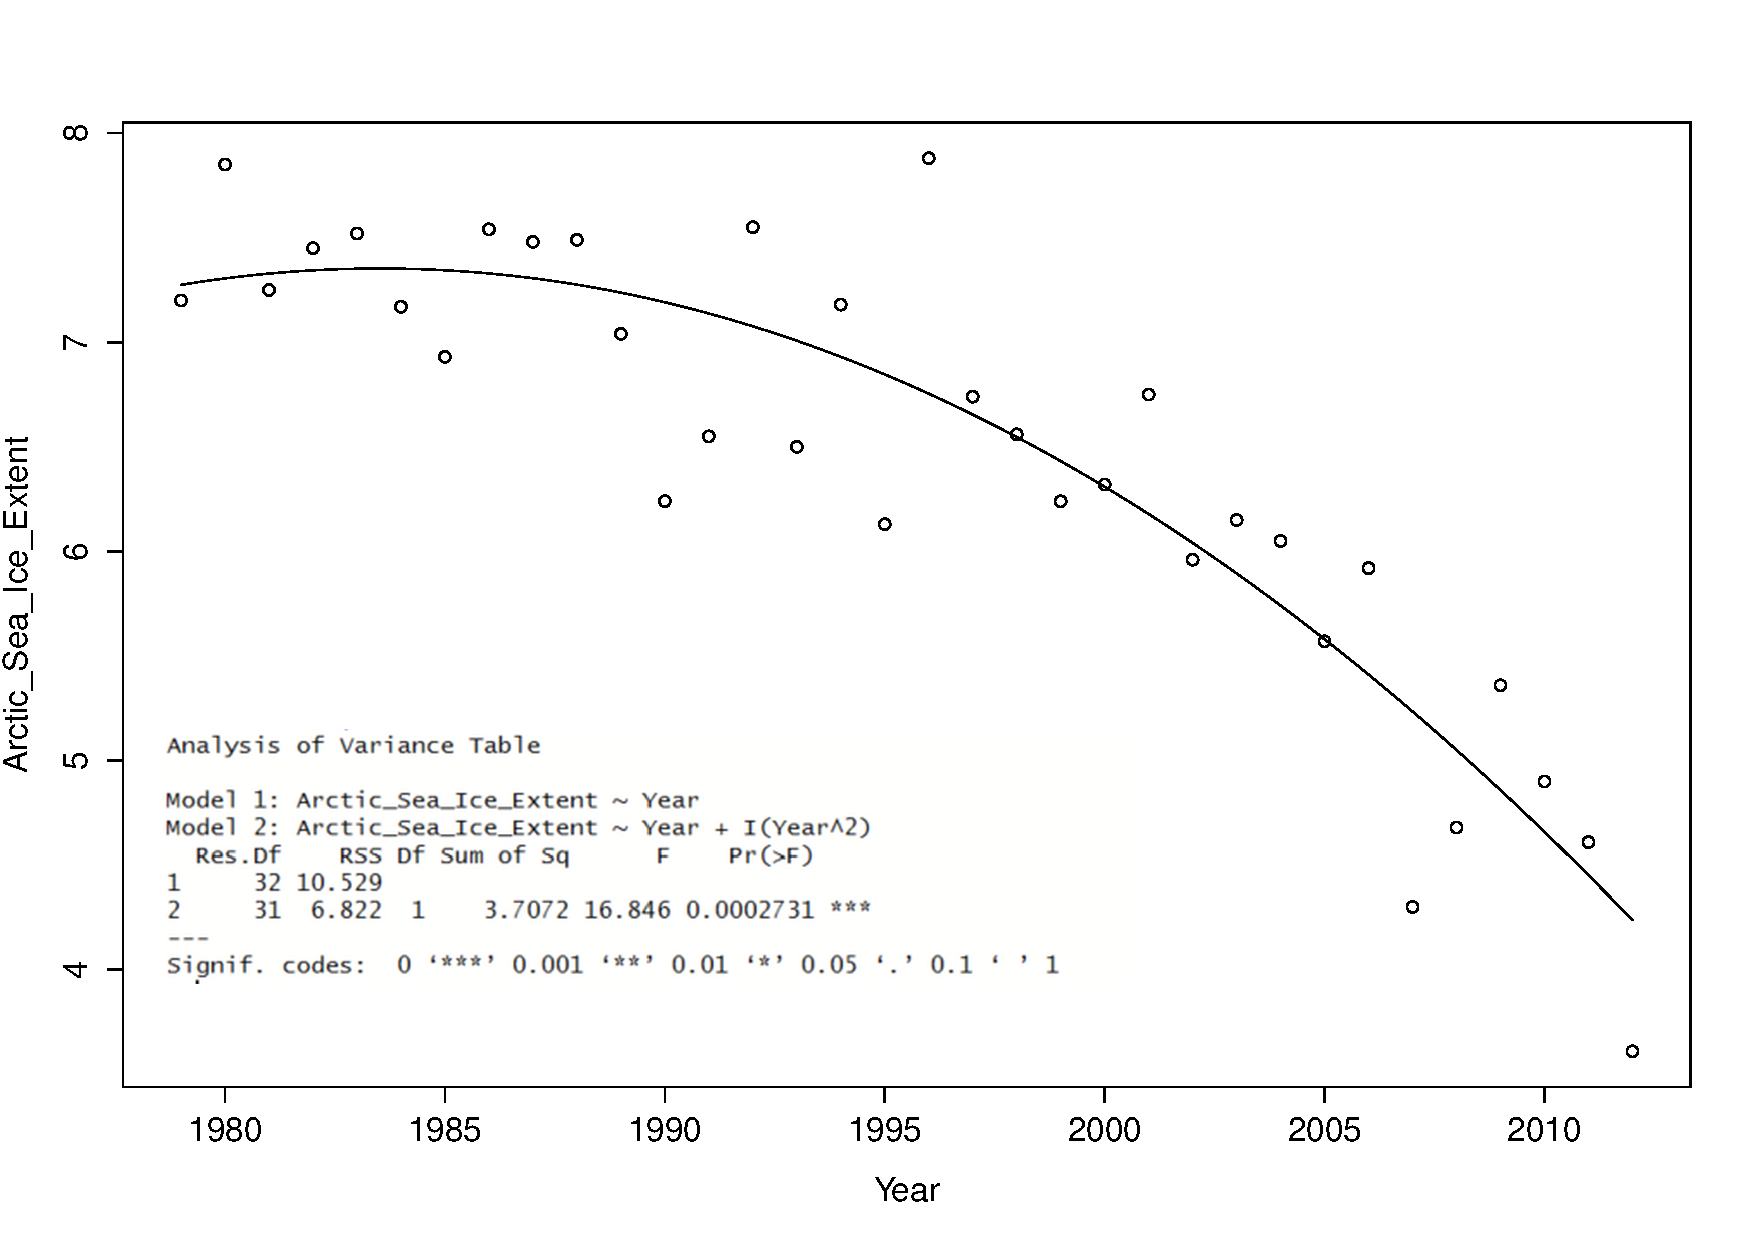
\includegraphics[width=0.8\textwidth]{sea_ice_quadratic2}
  \caption{Ajustement quadratique}
\end{figure}

\end{frame}





\end{document}
== 